%!TEX root = 2017-icip-provenance-filtering.tex
\section{Proposed Method}
\label{sec:method}
\label{sec:proposedmethod}

In this section, we present the proposed approach to provenance filtering. Given a query $q$, such as the image in the center of Fig.~\ref{provenance_mpp}, the objective is to search a collection of images $\mathcal{C}$ for all potential donors $r_i$ contributing to the creation of $q$, including possible near duplicates $r_{ij}$ of $r_i$. Near duplicates of $q$ are also of interest as they would be important for tracing the offspring of $q$ over time. 

\begin{figure}[t]
	\begin{center}
	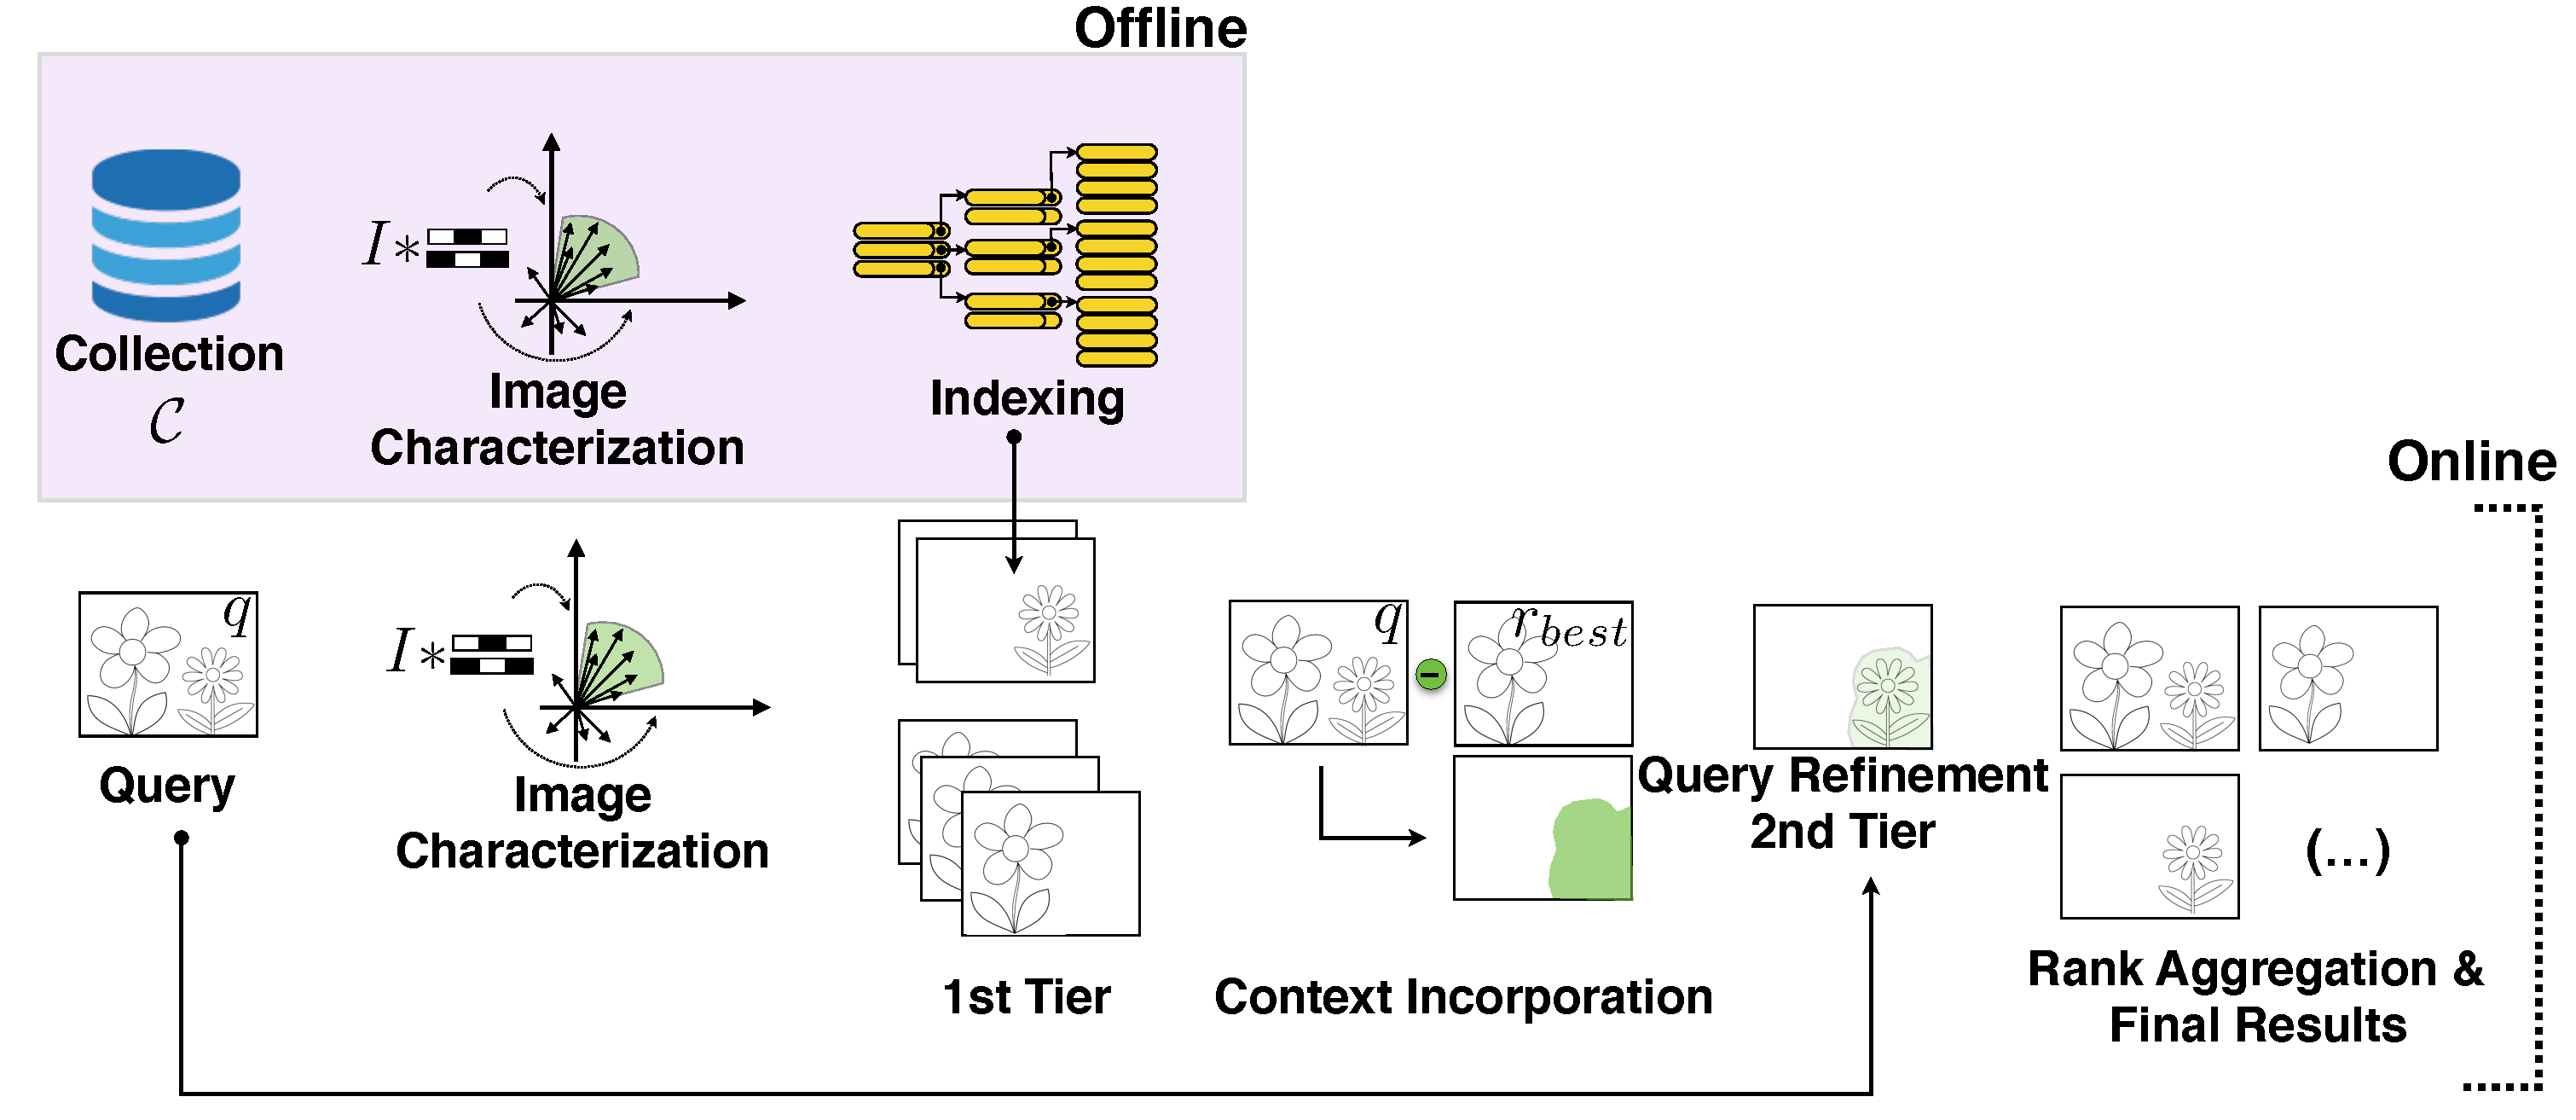
\includegraphics[width=0.95\columnwidth]{montage-pipeline-provenance-filtering}
	\caption{Method's pipeline. After retrieving related images, we compare the best result with $q$, incorporate the search's context and perform a second search to refine the list of possible donors.\label{fig:fig2}}	
	\end{center}
\end{figure}

Our approach to this problem involves two stages (c.f., Fig.~\ref{fig:fig2}). In the first stage, we design a fast image retrieval solution to recover the (likely) donor images, with high precision. We then exploit the context of the results to find the best match $r_{best}$ (respecting geometric constraints) with respect to $q$ and refine the donor list. Regions that are different between $q$ and its top-related image $r_{best}$ are of interest as they show regions that might have been incorporated into $q$ by combining pieces of different images in $\mathcal{C}$. Leveraging the contextual mask, the second stage of the search examines $\mathcal{C}$ a second time, focusing on finding potential localized donors. 

In the example of Fig.~\ref{provenance_mpp}, when querying the collection for potential donors (first tier/stage), we would likely retrieve the image with the table, flower and their background or the hand (as both are major contributors to the composite $q$). Calculating the contextual mask gives the region of the hand as a potential donor spliced from another source image(s). Therefore, when performing the second search, we look for images similar to that region, which would result in the donor for the hand as well as the other pieces. This process can be repeated a number of times if necessary. The different retrieved lists of results might be combined through rank aggregation techniques based on the confidence of the retrieved results. 

\subsection{Image Characterization}

The first step of our approach needs to represent each image in a robust manner so as to allow us retrieve partially related images in a large collection. In this context, using bags of words~\cite{Datta_2008} or deep learning techniques~\cite{Goodfellow_2016} would likely fail as they would be good for retrieving similar images in general but would not capture possible transformed donors, especially the small or heavily processed ones. In addition, a deep learning solution would require large image collections spanning different forgeries for a proper training and, in forensics, such collections are simply not available. In face of these limitations, we opted to represent each image using points of interest robust to image transformations, as forgeries often employ such transformations for more photorealistic montages. For that, we rely upon Speeded-Up Robust Features (SURF)~\cite{Bay:CVIU:2008}. We represent an image with about 2000 keypoints for small-scale experiments and with about 500 keypoints for large-scale ones. 

\subsection{Indexing Structure}
Given a query image $q$ and a collection of images $\mathcal{C}$ for searching, we need to represent the images in $\mathcal{C}$ in a very compact fashion so as to allow fast querying. For that, we use an indexing algorithm for finding nearest neighbors of $q$, in terms of their representative keypoints. More specifically, after extracting the points of interest for all images in $\mathcal{C}$, we need to find the $k$-nearest points to each keypoint in $q$. We further perform majority voting to infer the similarity between the query image $q$ and each image in $\mathcal{C}$ based on the nearest keypoints retrieved from the gallery.

As the number of points of interest extracted from $\mathcal{C}$ might reach hundreds of millions, the comparison between the $q$ and all images in $\mathcal{C}$ using brute-force search is impracticable. Therefore, we investigated some algorithms for $\epsilon$-approximated nearest neighbors, adequate for large-scale searches. According to Arya~\cite{Arya_1998}, an approximate search can be achieved by considering (1 + $\epsilon$)-approximate nearest neighbors for which $dist(k,l) \leq (1+\epsilon)dist(p,l)$ such that $p$ is the true nearest neighbor for $l$. Nonetheless, these solutions might lose effectiveness depending on the heuristic adopted to speed up the search. For this reason, here we compare four indexing approaches in terms of runtime, memory footprint and quality of the search: KD-Trees and KD-Forests~\cite{Bentley:COMMUN:1975}, Hierarchical Clustering~\cite{Steinbach:KDD:2000}, and Product Quantization~\cite{Jegou:TPAMI:2011}. 

\subsection{Context Incorporation and Ranking Aggregation}
To retrieve the donor images with high recall rates, we propose a query refinement process, referred to as context incorporation, in that we use the ranking result obtained in a first tier to reformulate the query so that small objects used to compose the spliced image can be be retrieved more accurately. First, we need to make sure the query is well represented in terms of describing keypoints. The overrepresentation of the query $q$ aims at guaranteeing we sample basically all of its regions, including the background. Although SURF descriptors are robust to describe objects in general in a scene, this approach most likely will fail in finding interest points inside very small objects, mainly when such objects are put in a complex background. To overcome this problem, we perform a query refinement by computing the intersection between $q$ and the best-matching retrieved image (most likely the host / background donor). This leads to a new query image containing just the information about the objects added in the host image. Our second search stage consists of querying the collection using the keypoints falling within the selected regions of interest. We combine the different ranked lists using the confidence of the retrieved images (number of votes and keypoints matched).%; the higher the number of summed votes, the better the position in the final ranked list).

\subsection{Finding the Contextual Mask}
To find the contextual mask, we perform an image registration between $q$ and the top-match image $r_{best}$ in the ranked list obtained in the first tier of search. We match SURF features extracted from both images, select the $25$ best-matching keypoints and calculate the distance between the two images using the selected pairs of matches. We then calculate the geometrical transformation present in $r_{best}$ with respect to $q$ via image homography. Next, we compute the mask that indicates the candidate regions in which we might have spliced objects. We generate this mask by computing the difference between geometrically aligned images, followed by an opening operation with a $5\times5$-structuring element and a $5\times5$-kernel median filter to reduce the residual noise present in the mask. We also perform color quantization to 32-bits before computing the difference between the two images to reduce the presence of noise in the mask. 

There are some extreme cases for this approach that are worth discussing. First, when the top retrieved image does not have anything in common with $q$, the calculated mask should be null. In this case, there should be no search in the second tier. In turn, when $q$ itself is not a composite, the top retrieved image might be non-related at all (case one above) or a near-duplicate of $q$, in which case the mask is virtually identical to $q$. In the latter case, the search in the second tier should result in basically the same images retrieved in the first tier. Fig.~\ref{fig:contextual:mask} depicts examples of a query $q$, its top result $r_1$ and the calculated contextual masks. 

\begin{figure}[t]
	\begin{center}
	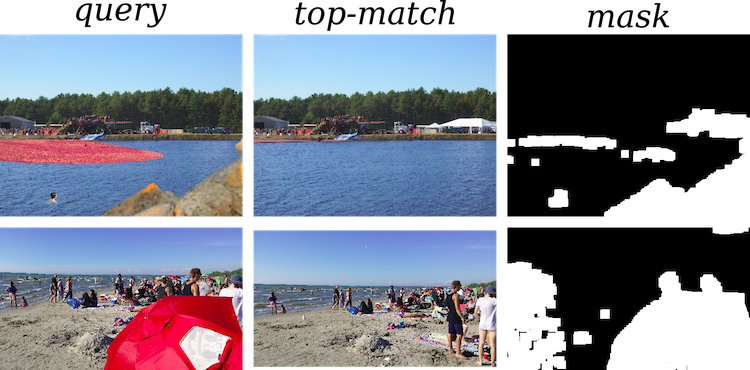
\includegraphics[width=0.6\linewidth]{contextual-mask}
	\caption{Example of a query, its top-related donor and the contextual mask. In the top row, the contextual mask captures the added rocks, person, bird and red-dirty region. In turn, the mask in the second row captures the added umbrella, content-smoothed sand on the left and the deleted white bird. 
	\label{fig:contextual:mask}}
	\end{center}
\end{figure}
